\chapter{NLP with DL}\label{sec:nlp}

\chapternote{Natural Language Processing with Deep Learning}{Stanford CS224n Winter 2019}

\begin{learningobjectives}
	\item Word Vector
	\item Calculus Review
	\item RNN \& Language Model
	\item Seq2Seq \& Attention
	\item ConvNet for NLP
	\item Transformer
\end{learningobjectives}

\dependencies{Machine Learning Basic}


\section{Word Vector}

Arguably the most simple word vector, i.e., \concept{one-hot vector}: an $\R^{|V| * 1}$ vector with one $1$ and the rest $0$s.
Note that these one-hot vectors are \concept{orthogonal} (i.e., no similarity/relastionship) and $V$ is a very big vocabulary ($\sim 500k$ words for english).

\sidenotedcmmc{In traditional NLP (before 2013), words are regarded as discrete symbols (\concept{localist} representation) and cannot capture similarity. One-hot vector is an example.}

Another idea: \concept{distributional representation} in modern statistical NLP. A word's meaning is given by the words that frequently appear close-by.
Using some $N$-dim ($N \ll |V|$) space is sufficient to encode all semantics of our language into a dense vector.
Once we get the word embedding matrix where each column is a word vector, we can query the word vector from one-hot representation by treating it as \concept{lookup table} instead of using matrix product.

\Figure{word_analogy}{An example of word analogy of man:woman :: king:?}

To evaluate word vectors, there are two fold: \emph{intrinsic} (directly used, e.g. word analogies/similarity) and \emph{extrinsic} (indirectly used in real task, e.g. Q\&A).
Word vector analygies for  $a:b :: c:\textcolor{red}{d}$ is calculated by cosine similarity as example shown in Fig.~\ref{fig:word_analogy}:

\begin{equation}
d = \arg \max_i \frac{(x_b - x_a + x_c)^\top x_i}{\lVert x_b - x_a + x_c \rVert}
\end{equation}

If we have hundreds of millions of words, it's okay to start the vectors \emph{randomly}.
If there is a \emph{small} ($\le 100,000$) training data set, it's best to just treat the pre-trained word vectors as \emph{fixed}.
In the other hand, if there is a large dataset, then we can gain by \concept{fine tuning} of the word vectors.

\subsection{Word2vec}

Two families of models: \concept{Skip-gram} and \concept{Continuous Bag of Words}.

Idea of \concept{Skip-gram} (predicting context words by a given center word) in  Word2vec\mycite{word2vec}:

\begin{itemize}
	\item a large corpus of text $T$ with a vocabulary $V$
	\item every word is represented by a vector $w \in \mathbb{R}^d$ and start off as a random vector
	\item use the (cosine) similarity of the word vectors for $c$ (center word) and $o$ (context/outside word) to calculate the probability of $o$ given $c$: $p(w_o | w_c)$
	\item adjusting the word vectors to maximize the probability
\end{itemize}

\sidenotedcmmc{Why we use two vectors per word? Make it simpler to calculate the gradient of loss function. Because the center word would be one of the choices for the context word and thus squared terms are imported. Average both vectors at the end is the final word vector.}

The conditional probability is calculated by the \concept{softmax} (normalize to probability distribution) of \concept{cosine} similarity (review dot product: $\bm{a} \cdot \bm{b} = |\bm{a}||\bm{b}| \cos\left<\bm{a}, \bm{b}\right>$).
Note that the visualization of word vectos utilizes 2D projection (e.g. PCA) that will loss huge information.

\begin{equation}
p(w_o | w_c) = \frac{\exp(u_o^\top v_c)}{\sum_{w \in V}(u_w^\top v_c)}
\end{equation}
where $v_c$ denotes the center word vector of $w$ when $w$ is used as a center word in the formula, and $u_w$ denotes the context word vector of $w$ as the similar way.
A demo of the window size and conditional probability is shown in Fig.~\ref{fig:word2vec:window_cond}.

\MoveNextFigure{+5cm}
\Figure{word2vec:window_cond}{A demo of the window size and $p(w_o | w_c)$}


The objective function (a.k.a loss or cost function) is given by the (average) negative log likelihood (abbr. \concept{NLL}).
The parameters of the model are adjusted by minimizing the loss function $J(\theta)$ or maximizing the likelihood.
This is, give a high probability estimate to those words that occur in the context and low probability to those don't typically occur in the context.


\begin{align}
	\arg\max_\theta L(\theta) &= \prod_{c=1}^{T} p(w_{c-m}, \cdots, w_{c-1}, w_{c+1}, \cdots, w_{c+m} | w_c; \theta) \nonumber \\
	&= \prod_{c=1}^{T} \prod_{\substack{-m \le j \le m \\ o = j + c \\ o \ne c}} p(w_o | w_c; \theta) \nonumber \\
	&\Downarrow \nonumber \\
	\arg\min_\theta -\frac{1}{T} \log L(\theta) &= -\frac{1}{T} \sum_{c=1}^{T} \sum_{ \substack{-m \le j \le m \\ o=j+c \\ o \ne c}} \log p(w_o | w_c; \theta) \nonumber \\
	&= -\frac{1}{T} \sum_{c=1}^{T} \sum_{ \substack{-m \le j \le m \\ o=j+c \\ o \ne c}} \left( u_o^\top v_c - \log \sum_{w \in V} \exp(u_w^\top v_c)\right) 
	\label{eq:word2vec_loss}
\end{align}
where $m$ is the window size, $\theta \in \mathbb{R}^{2d|V|}$ represents all model parameters.
And we assume that $p(\cdot | w_c)$ are \concept{i.i.d}.

\sidenotedcmmc{The properties of $\log$ and $\arg \max$ ($\arg \min$) used in Eq.~\ref{eq:word2vec_loss} are VERY useful. $\exp(\cdot)$ ensures anything positive.}

We use \concept{gradient descent} (i.e. averaged gradient of all samples/windows) to optimize the loss function.
Note that stochastic (one sample/window with noisy estimates of the gradients) or mini-batch (a subset of samples/windows with size powered of $2$ such as $64$) gradient descent methods are useful to prevent overfitting and train for large dataset.
Calculating the gradient of the loss function is trivial:

\begin{equation}
\begin{split}
\frac{\partial J}{\partial v_c} &= -\frac{1}{T} \sum_{c=1}^{T} \sum_{ \substack{-m \le j \le m \\ o=j+c \\ o \ne c}} \left(u_o - \sum_{x \in V} \frac{\exp(u_x^\top v_c) u_x}{\sum_w \exp(u_w^\top v_c)}\right) \\
&= -\frac{1}{T} \sum_{c=1}^{T} \sum_{ \substack{-m \le j \le m \\ o=j+c \\ o \ne c}} \left(u_o - \sum_{x \in V} p(w_x | w_c) \cdot u_x \right)
\end{split}
\end{equation}

\begin{equation}
\frac{\partial J}{\partial u_o} = -\frac{1}{T} \sum_{c=1}^{T} \sum_{ \substack{-m \le j \le m \\ o=j+c \\ o \ne c}} \left(v_c - p(w_o | w_c)\right)
\end{equation}

Iteratively update equation (na\"ive version) is given by:

\begin{equation}
\theta^{new} = \theta^{old} - \alpha \nabla_\theta J(\theta)
\end{equation}
where $\alpha$ is the learning size (step size) such as $10^{-3}$.

Note that the summation over $|V|$ ($\sum_{x \in V}$) is very expensive to compute!
For every training step, instead of looping over the entire vocabulary, we can just sample several negative examples!
\concept{negative sampling}: train binary logistic regression instead.
$p(D=1|w_o,w_c)$ denotes the probability when $(w_o,w_c)$ came from the same window pf the corpus data, and $p(D=0|w_o,\tilde{w}_o)$ is the probability given $(w_o,\tilde{w}_o)$ did not come from the same window (i.e. noisy/invalid pair).
Randomly sample a bunch of noise words from the \concept{unigram distribution} raised to the power of $3/4$: $p(w) = \nicefrac{U(w)^{3/4}}{Z}$, where $U(w)$ is the counts for every unique words (i.e. unigram) and $Z$ is the nomalization term.

To avoid high frequence effect of words such as \concept{of} and \concept{the}, one simple way is just lop off the first biggest component in the word vector.
The unigram with power of $3/4$ in word2vec is also a trick to handle the effect, where it decrease how often you sample very common words and increase how often you sample rare words.

The objective function is also come from NLL: 

\begin{equation}
J(\theta) = - \frac{1}{T} \sum_{c=1}^T \sum_{ \substack{-m \le j \le m \\ o=j+c \\ o \ne c}} \left( \log \sigma \left( u_o^\top v_c \right) + \sum_{j \sim p(w)} \left[ \log \sigma \left(-u_j^\top v_c\right) \right] \right)
\end{equation}
where \concept{sigmoid} function is $\sigma(x) = \frac{1}{1 + e^{-x}}$ which can be seen as the 1D (binary) version of softmax and used to output the probability, and $k$ is the number of negative samples such as $5$ and $15$.
Note that according to the symmetric property of sigmoid function we get: $P(D=0|\tilde{w}_j,w_c) = 1 - P(D=1|\tilde{w}_j,w_c) = \sigma \left(-u_j^\top v_c\right)$.

\sidenotedcmmc{Although word2vec model is fairly simple and clean, there are actually many tricks which aren't particularly theoretical.}

\concept{Continuous Bag of Words} (CBOW): predict center word from (bag of) context words.
Similar to Skip-gram, the objective function is formulated as:

\begin{align}
J &= -\frac{1}{T} \sum_{c=1}^{T} \log P (w_c | w_{c-m}, \cdots, w_{c-1}, w_{c+1}, \cdots, w_{c+m}) \\
&= -\frac{1}{T} \sum_{c=1}^{T} \log p (v_c | \hat{u}) \\
&= -\frac{1}{T} \sum_{c=1}^{T} \log \mathop{\textup{softmax}}\limits_{c}(v_c^\top \hat{u}) \\
&= -\frac{1}{T} \sum_{c=1}^{T} (v_c^\top \hat{u} - \log \sum_{j=1}^{|V|} \exp (v_j^\top \hat{u}))
\end{align}
where $\hat{u} = \frac{1}{2m} \sum_{ \substack{-m \le j \le m \\ o=j+c \\ o \ne c}} u_o$


Although word2vec can capture complex patterns beyond word similarity, it has inefficient usage of statistics (i.e. rely on sampling rather than directly use counts of words).

\subsection{HW1}

A simple intro to co-occurrence matrix, SVD, cosine similarity, and some applications (e.g. word analogy) of word2vec.

\subsection{GloVe}
\Figure{cooccurrence_matrix}{An example of co-occurrence matrix with window size of $1$}

Co-occurrence matrix $X \in \mathbb{R}^{|V| * |V|}$ with window size $k$.
Fig.~\ref{fig:cooccurrence_matrix} shows an example.
Note that such matrix is extremely sparse and very high dimensional, and the dimensions of the matrix change very often as new words are added very frequently and corpus changes in size.
We can perform SVD on $X$ to reduce the dimensionality to $25 \sim 1000$-dim.
In addition, there are some hacks to $X$ that transform the raw count introduced by \mycite{rohde2005_hacks}: (1) set upper bound (e.g. $100$) or just ignore them all for the counts of too frequent words, (2) ramped windows that count closer words more. (3) use Pearson correlations instead of counts.
Note that they made some interesting observation in their word vector that the verb (e.g. swim) and the corresponding doer (e.g. swimmer) pairs are roughly \emph{linear components} (e.g. $\bm{v}_{swimmer} - \bm{v}_{swim} = k (\bm{v}_{driver} - \bm{v}_{drive})$).

\tododcmmc{SVD}

Although the aforementioned conventional method has disproportionate importance given to large counts and mainly only capture word similarity, it enjoys the fast training and efficient usage of statistics.
GloVe (\textbf{Glo}bal \textbf{Ve}ctor) \mycite{GloVe} combines the advantages from both of this conventional method (global count matrix factorization) and the DL-based methods (local context window methods) such as word2vec.
It captures global corpus statistics directly.

\Figure{ratio_cooccurrence}{An example of the conditional probabilities and their ratio in GloVe paper.}

Some notations: $X_{ij}$ tabulate the number of times word $j$ occurs in the context of word $i$, $X_i = \sum_{k} X_{ik}$ is the number of times any word appears in the context of word $i$ i.e., the nomalization denominator.
$P_{ij} = P(j|i) = \nicefrac{X_{ij}}{X_i}$ is the probability that word $j$ appear in the context of word $i$.
The crucial insight is that the \emph{ratios} of co-occurrence probabilities as shown in Fig.~\ref{fig:ratio_cooccurrence} to encode meaning components.
We'd like to leverage the word vectors $w_i, w_j, \tilde{w}_k$ to represent such ratio: $F(w_i, w_j, \tilde{w}_k) = \nicefrac{P_{ik}}{P{jk}}$, where $\tilde{w}$ is a seperate \emph{context} word vector for various \emph{probe words} $k$, instead of the word vector $w$ (similar to center word vector in skip-gram).

We can select a unique choice of $F$ by enforcing a few desiderata (i.e. restrictions).
To fit the demand of the \emph{linear components} and the output \emph{scalar} value, in addition to the \emph{homomorphism}
between the groups $(\mathbb{R}, -)$ and $(\mathbb{R}^+, \div)$ (i.e., $F(i,j) = \nicefrac{P_{ik}}{P{jk}} = \nicefrac{1}{F(j,i)} = \nicefrac{P_{jk}}{P{ik}}$), we can derivate that $F(w_i, w_j, \tilde{w}_k) = F\left((w_i - w_j)^\top \tilde{w}_k\right) = \nicefrac{F(w_i^\top \tilde{w}_k)}{F(w_j^\top \tilde{w}_k)} = \nicefrac{P_{ik}}{P_{jk}}$.
Therefore, $F=\exp, w_i^\top \tilde{w}_k = \log(P_{ik}) = \log (X_{ik}) - \log (X_i)$.
Note that the symmetry property of co-occurrence: $X_{ik} = X_{ki}$.
We add two biases to restore the symmetry: $w_i^\top \tilde{w}_k + b_i + \tilde{b}_k = \log (X_{ik})$, where we can analogy that $b_i + \tilde{b}_j = \log X_{i}$.

More details, the relationship to the "global skip-gram" and the complexity refer to the original GloVe paper~\mycite{GloVe}.

\sidenotedcmmc{To handle the ill-defined $\log$ function when its argument be $0$ (its common that $X_{ij}=0$), the authors use the factorized log: $\log(X_{ik}) \rightarrow \log (1+X_{ik})$.}

\begin{align}
w_i \cdot w_j &= \log P(i|j) \\
w_x \cdot (w_a - w_b) &= \log \frac{P(x|a)}{P(x|b)}
\end{align}

Therefore, the ratios of co-occurrence probabilities is the \concept{log-bilinear model with vector differences}.
The final objective function is \emph{weighted} \concept{least squares} (MSE) for this regression problem.

\begin{equation}
	J = \sum_{i,j=1}^V f(X_{ij})\left(\bm{w}_i^\top \tilde{\bm{w}}_j + b_i + \tilde{b}_j - 
	log X_{ij}\right)^2
\end{equation}
where weighted function (is also a hyperparamter) is:

\begin{equation}
f(x) =
\begin{cases}
	\left(\frac{x}{x_{max}}\right)^\alpha & \text{if } x < x_{max} \\
	1 & \text{otherwise}
\end{cases}
\end{equation}
where $x_{max} = 100, \alpha = \nicefrac{3}{4}$ (\emph{empirical} value). 

\subsection{Word sense ambiguity}
Because most words have lots of meanings.
One crude way \mycite{huang-etal-2012-improving} is to cluster word windows around words, retrain with each
word assigned to multiple different clusters $\textsf{bank}_1$, $\textsf{bank}_2$, etc.
Another method \mycite{TACL_word_senses} is weighted sum of different senses of a word reside in a linear superposition, e.g.:

\begin{equation}
v_{\text{pike}} = \alpha_1 v_{\text{pike}_1} + \alpha_2 v_{\text{pike}_2} + \alpha_3 v_{\text{pike}_3}
\end{equation}
where $\alpha_i = \frac{f_i}{\sum_{j=1}^3 f_j}$ for frequency $f$.

The result is counterintuitive very well, because of the idea from \emph{sparse} coding you can actually separate out the senses.

\section{Math Backgrounds}
For \concept{multi-class classification} problem, \concept{NLL} (negative likelihood loss) is the objective function of \concept{Maximum Likelihood Estimate} (abbr, MLE):

\begin{equation}
J(\bm{\theta}) = - \sum_i \log p(y = y^{true}_i | \bm{x}_i; \bm{\theta})
\end{equation}

\concept{cross entropy} (distance measure) between (discrete) distribution $p$ and $q$ is more convenient way:

\begin{equation}
H(p, q) = - \sum_{c=1}^C p(c) \log q(c)
\end{equation}

However, in the multi-class (with single label) setting, the p(c) is the \concept{ground truth distribution} which has the \emph{one-hot} style (\concept{empirical distribution}), i.e. $p = [0, \cdots, 0, 1, 0, \cdots, 0]$ where $1$ at the right class and $0$ everywhere else.
Therefore, the \concept{cross entropy} in the multi-class classification is \emph{equal} to the NLL.

A simple $k$-class model example is \concept{dense layer} with \emph{softmax}:

\begin{equation}
	p(y|\bm{x}; \bm{\theta}) = softmax(\bm{W}_2 f(\bm{W}_1 \bm{x} + \bm{b}))
\end{equation}
where $\bm{\theta} = [\bm{W}_1, \bm{b}, \bm{W}_2]^\top $ are the parameters, $\bm{x} \in \mathbb{R}^m, \bm{W}_1 \in \mathbb{R}^{n * m}, \bm{b} \in \mathbb{R}^n, \bm{W}_2 \in \mathbb{R}^{k * n}$, $f(\cdot)$ is a kind of simple activate (non-linear) function to provide non-linearity, such as $ReLU(x) = max(0, x)$.
The visualization of neural network refer to \sidenote{ ConvNetJS: \url{https://cs.stanford.edu/people/karpathy/convnetjs/demo/classify2d.html}}.

The \concept{Jacobian Matrix} (generalization of the gradient) of function $\bm{f}(\bm{x}): \mathbb{R}^n \rightarrow \mathbb{R}^m$ is a $m \times n$ matrix: $\left(\frac{\partial \bm{f}}{\partial \bm{x}}\right)_{ij} = \frac{\partial f_i}{x_j}$.

Supposed that we have a function $\bm{g}(\bm{f}(x)), \bm{f}: \mathbb{R} \rightarrow \mathbb{R}^2, \bm{g}: \mathbb{R}^2 \rightarrow \mathbb{R}^2$, we can compute the partial derivative of $\bm{g}$ w.r.t $x$ by \concept{chain rule}:

\begin{equation}
	\frac{\partial \bm{g}}{\partial x} = \begin{bmatrix}
	\frac{\partial g_1}{\partial f_1} \frac{\partial f_1}{x} + \frac{\partial g_1}{\partial f_2} \frac{\partial f_2}{x}\\
	\frac{\partial g_2}{\partial f_1} \frac{\partial f_1}{x} + \frac{\partial g_2}{\partial f_2} \frac{\partial f_2}{x}
	\end{bmatrix}
\end{equation}

\sidenotedcmmc{$\frac{d g_1}{d \bm{y}} = \frac{\partial g_1}{y_1} + \frac{\partial g_2}{y_2}$ is the relationship of the full differential and the partial differential.}

It is the same as multiplying the two Jacobians:

\begin{equation}
\frac{\partial \bm{g}}{\partial x} = \frac{\partial \bm{g}}{\partial \bm{f}} \frac{\partial \bm{f}}{\partial x} = \begin{bmatrix}
\frac{\partial g_1}{\partial f_1} & \frac{\partial g_1}{\partial f_2} \\
\frac{\partial g_2}{\partial f_1} & \frac{\partial g_2}{\partial f_2}
\end{bmatrix} \begin{bmatrix}
\frac{\partial f_1}{\partial x} \\
\frac{\partial f_2}{\partial x}
\end{bmatrix}
\end{equation}

There are some useful identities:

\begin{itemize}
	\item $\frac{\partial \bm{x}}{\partial \bm{x}} = \bm{I}$
	\item $\frac{\partial \bm{Wx}}{\partial \bm{x}} = \bm{W}, \frac{\partial \bm{u}^\top \bm{x}}{\partial \bm{x}} = \bm{u}^\top$
	\item $\frac{\partial \bm{x^\top W}}{\partial \bm{x}} = \bm{W^\top}$
	\item For elemenwise function $\bm{f}(\bm{x})$: $\frac{\partial \bm{f}}{\partial \bm{x}} = \texttt{diag}(\bm{f}^\prime(\bm{x}))$
	\item $\frac{\partial \bm{\theta}^\top (\bm{W} \cdot \bm{h})}{\partial \bm{W}} = \bm{\theta} \bm{h}^\top$ where $\bm{\theta} \in \mathbb{R}^{D_\theta * 1}, \bm{W} \in \mathbb{R}^{D_\theta * D_h}, \bm{h} \in \mathbb{R}^{D_h * 1}$
	\item For cross entropy loss: $J(\bm{h}) = - \bm{y}^\top \log (\hat{\bm{y}}) = - \bm{y}^\top \log \texttt{softmax}(\bm{h})$ ($\bm{y}$ is one-hot vector) is: $\frac{\partial J}{\partial \bm{h}} = (\hat{\bm{y}} - \bm{y})^\top$
\end{itemize}

We can use \concept{backward propagation} (reversed of the \emph{topological sort}) and \emph{re-use} intermediate nodes to reduce complexity in the \emph{computation graph}.

Other machine learning basic concepts are: \concept{regularization} (e.g. L2) to prevent \concept{overfitting}, vectorization to parallelization, (non-linear) \concept{activation function} (e.g. sigmoid, tanh, (leaky) ReLU), parameter initialization (e.g. Xavier), \concept{Optimizer} (e.g. RMSprop, Adam), learning rate.

\sidenotedcmmc{Compared with activations such as sigmoid and tanh, ReLU does not \emph{saturate} even for larger values. Note that ReLU is not \emph{differentiable} at $0$, where we can use \emph{sub-derivatives} in implementation with a certain value such as $0$ or $1$.}

\subsection{Data Preprocessing}
\Figure{mean_subtraction}{An exmaple of mean subtration.}
\Figure{normalization}{An example of normalization.}

\begin{itemize}
	\item \textbf{Mean Subtraction (Shifting)}: Shifting all data so that they have zero mean as shown in Fig.~\ref{fig:mean_subtraction}. Formally, $\bm{x}^{(i)} \leftarrow \bm{x}^{(i)} - \mathbb{E}[\bm{x}^{(i)}]$ for sample $i$, where $\mathbb{E}$ indicates mean.
	\item \textbf{Normalization (Scaling)}: Scale every input feature dimension to have
	similar ranges of magnitudes, as shown in Fig.~\ref{fig:normalization}. This is useful since input features are often measured in different "units", but we often want to initially consider all features as equally important. Formally, $x^{(i)}_{j} \leftarrow \frac{x^{(i)}_{j}}{\sigma_i (x^{(i)}_{j})}$ for feature $j$ in sample $i$ where $\sigma(\cdot)$ is the standard variance over $x^{(0)}_{j}, \cdots, x^{(N)}_{j}$.
	\item \textbf{Whitening}: Whitening converts the data to a have an identity covariance matrix - that is, features become uncorrelated and have a variance of $1$. In the specific, we can divide the principal components achieved from PCA by the square roots of their eigenvalues (singular value).
\end{itemize}

\subsection{Parameter Initialization}
	
If two hidden units have exactly the same bias and exactly the same incoming and outgoing weights (e.g. different channels for learning different features in the same convolutional layer), they will always get exactly the same gradient.
So we should initialize the weights to small random values.

A good starting strategy is to initialize the weights to small random numbers of \concept{normal distribution} with the mean around $0$.
Xavier et al. \mycite{Xavier} suggest that for sigmoid and tanh activation units, it's better for the weight matrix $W \in \mathbb{R}^{n^{(l+1)} * n^{(l)}}$ to be initialized randomly with a \concept{uniform distribution}:
\begin{equation}
W \sim U\left[- \sqrt{\frac{6}{n^{(l)} + n^{(l+1)}}}, \sqrt{\frac{6}{n^{(l)} + n^{(l+1)}}}\right]
\end{equation}
where $n^{(l)}, n^{(l+1)}$ are also called \textbf{fan-in} and \textbf{fan-out}.
Besides, bias units are initialized to $0$.

\subsection{Optimizer}
To avoid a diverging loss (too large learning step) or unconverging (too small learning step), there are some learning strategies.

\concept{Annealing}: start off with a high learning rate to approach a minimum quickly, after several iterations, the learning rate is reduced in some way under a more fine-grained scope.
\begin{itemize}
	\item Exponential decay: $\alpha(t) = \alpha_0 e^{-kt}$ where $\alpha_0$ is initial learning rate.
	\item Decrease over time: $\alpha(t) = \nicefrac{(\alpha_0 \tau)}{\max(t, \tau)}$ where $\tau$ denotes the time at which the learning rate should start reducing.
\end{itemize}

\Figure{momentum}{A picture of momentum.}

\concept{Momentum} (a picture of it can be seen in Fig.\ref{fig:momentum}) based methods:
\begin{itemize}
	\item AdaGrad: $\bm{m} \leftarrow \bm{m} + \left(\nabla_{\bm{\theta}} J (\bm{\theta})\right)^2, \bm{\theta} \leftarrow \bm{\theta} - \alpha \nabla_{\bm{\theta}} J (\bm{\theta}) \odot \left(\sqrt{\bm{m}} + \epsilon\right)^{-1}$ where $\odot, (\cdot)^{-1}, (\cdot)^{2}, \sqrt{\cdot}$ are all element-wise operators, and $\epsilon$ is a very small value such as $10^{-8}$ to prevent \concept{arithmetic underflow}.
	It leads to that parameters that have not been updated much in the past are likelier to have higher learning rates now.
	\item RMSprop: $\bm{m} \leftarrow \beta \bm{m} + (1-\beta) \left(\nabla_{\bm{\theta}} J (\bm{\theta})\right)^2, \bm{\theta} \leftarrow \bm{\theta} - \alpha \nabla_{\bm{\theta}} J (\bm{\theta}) \odot \left(\sqrt{\bm{m}} + \epsilon\right)^{-1}$ where $\beta$ is the decay rate with default value $0.9$. Unlike AdaGrad, its updates do not become monotonically smaller.
	\item Adam\mycite{Adam}: $\bm{m} \leftarrow \beta_1 \bm{m} + (1-\beta_1) \nabla_{\bm{\theta}} J (\bm{\theta}), \bm{v} \leftarrow \beta_2 \bm{v} + (1-\beta_2) \left(\nabla_{\bm{\theta}} J (\bm{\theta})\right)^2, \hat{\bm{m}} = \bm{m} / (1 - \beta_1^t), \hat{\bm{v}} = \bm{v} / (1 - \beta_2^t), \bm{\theta} \leftarrow \bm{\theta} - \alpha \hat{\bm{m}} /  \left(\sqrt{\hat{\bm{v}}} + \epsilon\right)^{-1}$, where $/$ is also a element-wise operator, hyperparameters $\beta_1 = 0.9, \beta_2 = 0.999 \in [0, 1)$. $\hat{\bm{m}}, \hat{\bm{v}}$ are the bias-corrected $\bm{m}, \bm{v}$, and they indicate a rolling average
	of the gradients and a rolling average of the magnitudes of the gradients, respectively. In adition, $\bm{m}, \bm{v}$ are all initialized to $\bm{0}$ Adam is like a combination of RMSProp and momentum.
\end{itemize}

\sidenotedcmmc{For the implementation of momentum such as RMSprop, there is a interesting small trick: use $\bm{m} = \bm{m} - (1-\beta)(\bm{m} - \left(\nabla_{\bm{\theta}} J (\bm{\theta})\right)^2)$ instead of $\bm{m} = \beta \bm{m} + (1-\beta) \left(\nabla_{\bm{\theta}} J (\bm{\theta})\right)^2$. In such way, we need calculate only one multiplication, compared with original two multiplications.}

\subsection{Regularization}
\textbf{1. Dropout}

During training, \concept{dropout} \mycite{dropout} randomly disables units in the hidden layer by a mask vector drawn from Bernoulli distribution where each entry is $0$ with probability $p_{\text{drop}}$ and $1$ with probability ($1 - p_{\text{drop}}$):
\begin{equation}
\text{Dropout Layer: } \textcolor{red}{d_i \sim \text{Bernoulli}(1 - p_{\text{drop}}), \hat{\bm{h}}^{(t)} = } \textcolor{blue}{\frac{1}{1-p_{\text{drop}}}} \textcolor{red}{\bm{d} \odot \bm{h}^{(t)}}
\end{equation}
where $\odot$ is element-wise product, $\bm{d} \in \{0, 1\}^{D_h}, \bm{h}^{(t)} \in \mathbb{R}^{D_h}$.

If the expected output of a neuron during testing if far different as it was during training, the magnitude of the outputs could be radically different, and the behavior of the network is no longer well-defined.
Therefore, all the parameters should divided by retain rate $1-p$ (blue part in above formula), so that $\mathbb{E}_{p_{\text{drop}}} [\bm{h}_{\text{drop}}]_i = h_i$.
If we do not such correction in training, we should multiply $1-p$ to all related parameters.

If we use dropout in testing, the result is \emph{unstable} (vary from every testing) because of the
dropout is drawn from Bernoulli distribution.
Therefore, we should apply dropout only during training but not during evaluation or testing.

A motivation of dropout is to reduce complex \emph{co-adaptations} among the hidden units which comes from the superiority of sexual reproduction compared with asexual.
The criterion for natural selection may be the mix-ability of genes.
A gene which rely only on a \emph{small} number of other genes is able to work well with another random set of genes that could come from another paraent's genes in sexual reproduction.
Hence, it will more robust aginst noises and increases the chance of a new gene improving the fitness of an individual.

\textbf{2. Batch Normalization}

Although \concept{batch nomalization} \mycite{BatchNorm} is like nomalization used in data preprocessing with $N$ be the mini-batch size instead of the dataset size, it is inserted between hidden layers to normalize the output of last layer.
It leads to achieve the fixed distributions of inputs that would remove the ill effects of the internal covariate shift.
\emph{Internal Covariate Shift} is defined as the change in the distribution of network activations due to the change in network parameters during training.

The batch normalization in training is defined as follows:
\begin{equation}
\text{BN}(h_i) = \gamma \frac{h_i - \mu_{\mathcal{B}}}{\sqrt{\sigma_{\mathcal{B}}^2 + \epsilon}} + \beta
\end{equation}
where $\gamma, \beta$ are \concept{trainable parameters}, $\mu_{\mathcal{B}}, \sigma_{\mathcal{B}}^2$ are the mean and variance over the mini-batch as the way of normalization for data preprocessing.
Since the mean subtraction will \emph{ignore} the learned bias which may useful to the model.
The trainable $\gamma$ and $\beta$ are used to corrected them and make the BN layer trainable.
Them ensure that the batch normalization inserted in the network can represent the identity transform.

However, when testing, we cannot use mini-batch in most time.
We instead feed one sample into the model.
Therefore, we leverage $m$ training mini-batches to perform \concept{unbiased estimates} of them:
\begin{align}
&\mathbb{E}[h_i] \leftarrow \mathbb{E}_{\mathcal{B}}[\mu_{\mathcal{B}}] \nonumber \\
&\texttt{Var}[h_i] \leftarrow \frac{m}{m-1} \mathbb{E}_{\mathcal{B}}[\sigma_{\mathcal{B}}^2] \nonumber
\end{align}

Note that in many implementations, the above estimation is replaced with the way like the momentum used in RMSprop.
More details refer to the source code, e.g. Keras.
For the motivation, the use of BatchNorm makes models much less sensitive to parameter initialization.

\subsection{Practice: Named Entity Recognition}
To find and classify words as entities (e.g. location, or organization) in text.
One simple idea is that train softmax classifier to classify a center word by taking
\emph{concatenation} of word vectors surrounding it in a window (\emph{word window}) \mycite{NER_ICML}.
To perform NER of localtion, we need (unnormalized) score for each window, and make \emph{true window}’s (i.e. location in the center) score larger and other \emph{corrupt window}’s score lower.
The model is formulated as:

\begin{equation}
s = \bm{W}_2 f(\bm{W}_1 \bm{x} + \bm{b})
\end{equation}


The objective function (\emph{max-margin loss}) is:

\begin{equation}
J = max(0, s_c - (s - 1))
\end{equation}
where $s$ and $s_c$ is the score of true window and corrupt window.
It ensure each window with an NER location at its center should have a score $+1$ higher than any window without a location at its center.

\subsection{HW2}

Gradient calculation and implementation of word2vec.

\textbf{1. Written: Understanding word2vec}
\begin{align*}
	&(a) \ \hat{y}_o = P(O = o | C = c) \\
	&(b) \ \frac{\partial J}{\partial \bm{v}_c} = (\hat{\bm{y}} - \bm{y})^\top \bm{U}^\top \\
	&(c) \ \frac{\partial J}{\partial \bm{U}} = \bm{v}_c (\hat{\bm{y}} - \bm{y})^\top \\
	&(d) \ \sigma (\bm{x}) = \frac{1}{1 + \exp (- \bm{x})}, \frac{d \sigma (\bm{x})}{\bm{x}} = \texttt{diag} (\sigma (x_i) (1 - \sigma (x_i))) \\
	&(e) \ \frac{\partial J}{\partial \bm{v}_c} = \sum_k \sigma (\bm{u}_k^\top \bm{v}_c) \bm{u}_k^\top - (1 - \sigma (\bm{u}_o^\top \bm{v}_c)) \bm{u}_o^\top \\
	& \ \frac{\partial J}{\partial \bm{u}_o} = (\sigma (\bm{u}_o^\top \bm{v}_c) - 1) \bm{v}_c^\top \\
	& \ \frac{\partial J}{\partial \bm{u}_k} = \sigma (\bm{u}_k^\top \bm{v}_c) \bm{v}_c^\top \\
	&(f) \ (i) \frac{\partial J}{\partial \bm{U}} = \sum_o \bm{v}_c (\hat{\bm{y}}_o - \bm{y}_o)^\top \\
	&(ii) \frac{\partial J}{\partial \bm{v}_c} = \sum_o (\hat{\bm{y}}_o - \bm{y}_o)^\top \bm{U}^\top \\
	&(iii) \frac{\partial J}{\partial \bm{v}_w} = \bm{0}
\end{align*}

\sidenotedcmmc{Use shape convention to check the result.}

\textbf{2 Coding: Implementing word2vec}

Note that $\bm{U}, \bm{V}$ in the handout are the matrices whose $i$-th column is the $n$-dimensional embedded vector for word $w_i$.
However, in the codes of HW2, all the centerWordVectors and outsideVectors are as rows.

\section{Dependency Parser}
Two views of linguistic structure: (1) constituency (i.e., phrase structure grammar, or context-free grammar) (2) Dependency structure.
Dependence parse trees (single root with optional fake root, acyclic) use binary asymmetric relations which depicted as typed arrows going from \emph{head} to \emph{dependent}.
Note that the natural language is ambiguity.

Basic transition-based dependency parser \mycite{nivre-2003-efficient} with stack $\sigma = [\text{ROOT}]$, buffer $\beta = w_1, \cdots, w_n$, set of dependency arcs $A = \emptyset$, and a set of actions (\emph{transitions}) based on the above $3$-tuple:
\begin{align}
&\text{1. Shift: } \sigma , w_i | \beta, A \Rightarrow \sigma | w_i, \beta, A \nonumber \\
&\text{2. Left-Arc reduction: } \sigma | w_i | w_j, \beta, A \Rightarrow \sigma | w_j, \beta, A \cup \{r(w_j, w_i)\} \nonumber \\
&\text{3. Right-Arc reduction: } \sigma | w_i | w_j, \beta, A \Rightarrow \sigma | w_i, \beta, A \cup \{r(w_i, w_j)\} \nonumber
\end{align}
where $r(w_j, w_i)$ denotes $w_i$ is the dependency of $w_j$ (e.g. $\text{nsubj}(\text{ate} \rightarrow \text{I})$), $|$ and $\cup$ stand for concatenate.
The finish state is: $\sigma = [w], \beta = \emptyset$.
How to select (search) the best choice among the exponential size of different possible parse trees is the problem.
In 1960s, they use \emph{dynamic programming algorithms} ($\mathcal{O}(n^3)$).
In paper \mycite{nivre-2003-efficient}, the authors predict each action by a discriminative classifier (e.g. SVM classifier) which is more efficient but the accuracy is fractionally below the state-of-the-art.

\subsection{Neural Dependency Parsing}
Compared with traditional sparse feature-based discriminative dependency parsers, the work by \mycite{chen-manning-2014-fast} utilizes \concept{feedforward neural network model} with simple \concept{dense layers} and the softmax layer to predict each transition.
The input features with embedding dimension $d$ are:

\begin{enumerate}
	\item $x^{w} \in \mathbb{R}^{d * N_w}$: The top $3$ words on the stack and buffer $s_1, s_2, s_3, b_1, b_2, b_3$; the first and second leftmost / rightmost children of the top two words on the stack $lc_1(s_i), rc_1(s_i), lc_2(s_i), rc_2(s_i), i = 1, 2$; the
	leftmost of leftmost / rightmost of rightmost children of the top two words on the stack $lc_1(lc_1(s_i)), rc_1(rc_1(s_i)), i = 1, 2$; In total, $N_w = 18$.
	\item $x^{t} \in \mathbb{R}^{d * N_t}$: The corresponding POS (Part-of-speech, e.g. noun, verb, adjective) tags for $S_{word}$, $N_t = 18$.
	\item $x^{l} \in \mathbb{R}^{d * N_l}$:  The corresponding arc labels of words, excluding those $6$ words on the stack/buffer, $N_l = 12$.
\end{enumerate}

\sidenotedcmmc{Note that we use a special \textbf{NULL} token for non-existent elements: when the stack and buffer are empty or dependents have not been assigned yet.}

The predicted class is the one of transitions (i.e. shift, left/right arc reduction): $p = \texttt{softmax}(\bm{W}_2 f(\bm{W}_1^w \bm{x}^w + \bm{W}_1^t \bm{x}^t + \bm{W}_1^l \bm{x}^l + \bm{b}_1) + \bm{b}_2)$, where $f(\cdot)$ is the activation function (e.g. ReLU, or $x^3$).
The number of class is $3$ when untyped reductions or $T * 2 + 1$ when typed reductions (e.g. left-arc reduction with type \emph{nsubj}).

Here are mainly four types of parsing error:
\begin{itemize}
	\item \textbf{Prepositional Phrase Attachment Error}
	\item \textbf{Verb Phrase Attachment Error}
	\item \textbf{Modifier Attachment Error}
	\item \textbf{Coordination Attachment Error}
\end{itemize}

\subsection{HW3}
\textbf{1. Machine Learning \& Neural Networks}

\begin{enumerate}[label=(\alph*)]
	\item Adam
	\begin{enumerate}[label=(\roman*)]
		\item Because $\beta = 0.9$, most of the final gradients ($\bm{m}$) come from the past ($90\%$). Even if current gradients are varying much from previous, it only occupy $1 - \beta_1 = 0.1$ of the final gradients.
		\item Parameters that have not been updated much in the past are likelier to have higher learning rates.
	\end{enumerate}
	\item Dropout
	\begin{enumerate}[label=(\roman*)]
		\item If the expected output of a neuron during testing if far different as it was during training, the magnitude of the outputs could be radically different, and the behavior of the network is no longer well-defined. Thus, all the parameters should divided by retain rate $1-p$, so that $\mathbb{E}_{p_{\text{drop}}} [\bm{h}_{\text{drop}}]_i = h_i$.
		\item If we use dropout in testing, the result is unstable because of the dropout is drawn from Bernoulli distribution.
	\end{enumerate}
\end{enumerate}

\textbf{2. Neural Transition-Based Dependency Parsing}

(a) The remaindered configuration is:
\begin{table}
	\begin{center}
		\begin{tabular}{c|c|c|c}
			Stack & Buffer & New dependency & Transition \\
			\hline
			[ROOT, parsed, this] & [sentence, correctly] & & \textsf{SHIFT} \\ \hline
			[ROOT, parsed, this, sentence] & [correctly] & & \textsf{SHIFT} \\ \hline
			[ROOT, parsed, sentence] & [correctly] & sentence $\rightarrow$ this & \textsf{LEFT-ARC} \\ \hline
			[ROOT, parsed] & [correctly] & parsed $\rightarrow$ sentence & \textsf{RIGHT-ARC} \\ \hline
			[ROOT, parsed, correctly] & [] & & \textsf{SHIFT} \\ \hline
			[ROOT, parsed] & [] & parsed $\rightarrow$ correctly & \textsf{RIGHT-ARC} \\ \hline
			[ROOT] & [] & ROOT $\rightarrow$ parsed & \textsf{RIGHT-ARC}
		\end{tabular}
	\end{center}
\end{table}

(b) $2n$

(e) dev UAS: 88.56, test UAS: 89.07

(f) Refer to \href{https://corenlp.run/}{Stanford CoreNLP} to visualize the results of dependencies parses (also may contain errors).
\begin{enumerate}[label=(\roman*)]
	\item Verb Phrase Attachment Error, wedding -> fearing should be heading -> fearing.
	\item Coordination Attachment Error, makes -> rescue should be rush -> rescue.
	\item Prepositional Phrase Attachment Error, named -> Midland should be guy -> Midland.
	\item Modifier Attachment Error, elements -> most should be crucial -> most.
\end{enumerate}

Note that in the source code, the restriction that the version of PyTorch must be 1.0.0 is meaningless and thus I remove it.

\section{Language Modeling and Recurrent Neural Networks}

Language Modeling: given a sequence of words $\bm{x}^{(1)}, \cdots, \bm{x}^{(t)}$, compute the probability distribution of the next word at $\bm{x}^{(t+1)}$:
\begin{equation}
P(\bm{x}^{(t+1)} | \bm{x}^{(1)}, \cdots, \bm{x}^{(t)})
\end{equation}

The joint probability of a text is:
\begin{equation}
P(\bm{x}^{(1)}, \cdots, \bm{x}^{(T)}) = \prod_{t=1}^T P(\bm{x}^{(t)} | \bm{x}^{(t-1)}, \cdots, \bm{x}^{(1)})
\end{equation}

$n$-gram is a chunk of $n$ consecutive words: unigram, bigram, trigram, 4-gram, ...
$n$-gram language model is based on a simplifying assumption: $\bm{x}^{(t+1)}$ depends only on the preceding $n-1$ words with i.i.d.:
\begin{align}
P(\bm{x}^{(t+1)} | \bm{x}^{(t)}, \cdots, \bm{x}^{(1)}) &= P(\bm{x}^{(t+1)} | \bm{x}^{(t)}, \cdots, \bm{x}^{(t-n+2)}) \nonumber \\
&= \frac{P(\bm{x}^{(t+1)}, \bm{x}^{(t)}, \cdots, \bm{x}^{(t-n+2)})}{P(\bm{x}^{(t)}, \cdots, \bm{x}^{(t-n+2)})} \nonumber
\end{align}
where the $n$-gram and (n-1)-gram probabilities are calculated by \emph{counting}.
There are some \emph{sparsity problems} with the above $n$-gram models such as the numerator or denominator is zero.
Some tricks such as \emph{smoothing} (add small $\delta$ to the count) and \emph{backoff} (e.g. $4$-gram backoff to $3$-gram) are proposed to solve them.

\begin{figure}[!thp]
	\centerline{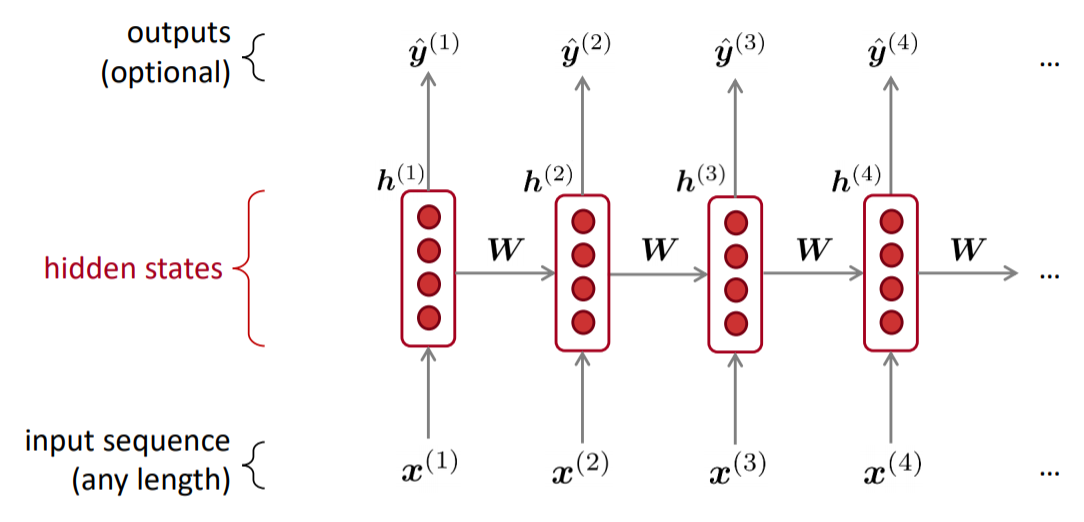
\includegraphics[width=8.0cm]{figs/RNN.png}}
	\caption{Principle of RNN}
	\label{RNN}
\end{figure}

\sidenotedcmmc{Note that for $n$-gram, increasing $n$ makes sparsity problems worse. Typically $n \le 5$.}

To process \emph{variable} length \concept{sequential input} such as text, \concept{Recurrent Neural Network} (RNN) is introduced.
As the principle of RNN shown in Fig.~\ref{RNN}: \emph{repeat} (i.e. \concept{unfold} or unroll) the same RNN cell for each time-step but with different input and previous \concept{hidden state}.
A vanilla RNN for language modeling is:
\begin{align}
\bm{h}^{(t)} &= \sigma \left(\bm{W}_h \bm{h}^{(t-1)} + \bm{W}_x \bm{x}^{(t)} + \bm{b}_1\right) \nonumber \\
\hat{\bm{y}} &= P(\bm{x}^{(t)} | \bm{x}^{(t-1)}, \cdots, \bm{x}^{(1)}) \nonumber \nonumber \\
&= \texttt{softmax}(\bm{U}\bm{h}^{(t)} + \bm{b}_2) \nonumber
\end{align}
where $\sigma(\cdot)$ is the activation function, and $\bm{h}^{(0)}$ is the initial (random or zero) hidden state.
The gradient w.r.t. the weight matrix is the \emph{sum} of the gradients w.r.t each time it appears using \concept{back-propagation through time} (BPTT, just as same as normal back-prop).
And the \concept{evaluation metric} for language modeling is \emph{perlexity} which is equal to the exponential of the cross-entropy losses:
\begin{align}
\text{perplexity} &= \prod_{t=1}^T \left(\frac{1}{P_{LM} (\bm{x}^{(t+1)} | \bm{x}^{(t)}, \cdots, \bm{x}^{(1)})}\right)^{\nicefrac{1}{T}} \nonumber \\
&= \exp\left(\frac{1}{T} \sum_{t=1}^T -\log \hat{\bm{y}}^{(t)}\right)
\end{align}

There are some other applications of RNN: part-of-speech tagging, named entity recognition, sentence classification, text generator, encoder module, etc.
The final feature can be the final hidden state or elemen-wise max/mean of all hidden states.
Using chain rule, we get $\frac{\partial J^{(n)}}{\partial \bm{h}^{(1)}} = \frac{\partial J^{(n)}}{\partial \bm{h}^{(n)}} \times \prod_{i=2}^n \frac{\partial \bm{h}^{(n)}}{\partial \bm{h}^{(n-1)}} = \frac{\partial J^{(n)}}{\partial \bm{h}^{(n)}} \times \prod_{i=2}^n \sigma^\prime \circ \bm{W}_h$.
For a large $n$ and small $\bm{W}_h$, it's easy to encounter the vanishing gradient problem.
In overall, the \emph{vanilla} RNN has these disadvantages: (1) recurrent computation is slow (2) hard to access long-term information (\concept{long-term dependencies}) due to \emph{gradient vanish} and \emph{gradient explosion}.

We can formalize the above vanishing intuitions according to \mycite{RNN_vanishing}.
Let $\bm{W}_h$ have the \concept{eigenvalues} $\lambda_1, \cdots, \lambda_n$ such that $|\lambda_1| > |\lambda_2| > \cdots > |\lambda_n|$ and the corresponding (left) eigenvectors $\bm{q}_1^\top, \cdots, \bm{q}_n^\top$ which have unit norms: $\bm{q}_i^\top \bm{W}_h = \lambda_i \bm{q}_i$.
We can rewrite the gradients $\frac{\partial J^{(n)}}{\partial \bm{h}^{(n)}} = \sum_{i=1}^N c_i \bm{q}_i^\top$ where $c_i = 0$ for $i < j$ and $c_j \ne 0$.
Thus, the overall gradient is:
\begin{align}
\frac{\partial J^{(n)}}{\partial \bm{h}^{(1)}} &= \frac{\partial J^{(n)}}{\partial \bm{h}^{(n)}} \times \prod_{i=2}^n \sigma^\prime \circ \bm{W}_h \nonumber \\ 
&= \sum_{i=1}^N c_i \bm{q}_i^\top (\texttt{diag}(\sigma^\prime))^{n-1} (\bm{W}_h)^{n-1} \nonumber \\
&= \sum_{i=1}^N c_i \bm{q}_i^\top (\bm{W}_h)^{n-1} (\texttt{diag}(\sigma^\prime))^{n-1} \nonumber \\
&= c_j \lambda_j^{n-1} \bm{q}_j^\top (\texttt{diag}(\sigma^\prime))^{n-1} + \lambda_j^{n-1} \sum_{i=j+1}^N c_i \left(\frac{\lambda_i}{\lambda_j}\right)^{n-1} \bm{q}_i^\top  (\texttt{diag}(\sigma^\prime))^{n-1} \nonumber \nonumber \\
&\approx c_j \lambda_j^{n-1} (\sigma^\prime)^{n-1} \bm{q}_j^\top \nonumber
\end{align}
where $\frac{\lambda_i}{\lambda_j} < 1$, and for large $n$ we have $\lim_{n \to \infty} \left(\frac{\lambda_i}{\lambda_j}\right)^{n-1} = 0$.
Therefore, if $\forall j, \sigma^\prime < \frac{1}{\lambda_j}$ then we get vanishing gradient.
Note that, $\sup(\text{sigmoid}^\prime) = \frac{1}{4}, \sup(ReLU^\prime) = 1$.
Thus, the largest eigenvalue $\lambda_1 < \frac{1}{\sigma^\prime}$ will lead to vanishing.

For avoid gradient explosion, one simple method is \emph{gradient clipping}: $\hat{\bm{g}} \leftarrow \frac{threshold}{\lVert \bm{g} \rVert} \bm{g}$ if $\lVert \bm{g} \rVert \ge threshold$.
As for fixing vanishing gradient, many RNN variants are introduced such as \concept{Long Short-Term Memory} (LSTM) \mycite{LSTM} and \concept{Gated Recurrent Unit} (GRU) \mycite{GRU}.
LSTM uses two \emph{separated} memories: \emph{hidden state} $\bm{h}^{(t)}$ for \emph{short-term} information and \emph{cell state} $\bm{c}^{(t)}$ for \emph{long-term} information.
There are three \emph{gates} performed in each LSTM \emph{cell}:
\begin{align}
&\text{Forget gate: } \bm{f}^{(t)} = \sigma(\bm{W}_f \bm{h}^{(t-1)} + \bm{U}_f \bm{x}^{(t)} + \bm{b}_f) \nonumber \\
&\text{Input gate: } \bm{i}^{(t)} = \sigma(\bm{W}_i \bm{h}^{(t-1)} + \bm{U}_i \bm{x}^{(t)} + \bm{b}_i) \nonumber \\
&\text{Output gate: } \bm{o}^{(t)} = \sigma(\bm{W}_o \bm{h}^{(t-1)} + \bm{U}_o \bm{x}^{(t)} + \bm{b}_o) \nonumber \\
&\text{New cell content: } \tilde{\bm{c}}^{(t)} = \tanh \left(\bm{W}_c \bm{h}^{(t-1)} + \bm{U}_c \bm{x}^{(t)} + \bm{b}_c \right) \nonumber \\
&\text{Cell state: } \bm{c}^{(t)} = \bm{f}^{(t)} \circ \bm{c}^{(t-1)} + \bm{i}^{(t)} \circ \tilde{\bm{c}}^{(t)} \nonumber \\
&\text{Hidden state: } \bm{h}^{(t)} = \bm{o}^{(t)} \circ \tanh \bm{c}^{(t)} \nonumber
\end{align}
where $\sigma$ is sigmoid function, $\circ$ is element-wise product, and $\tanh$ used in hidden state (the last formula) is to provide non-linearity and normalize $\bm{c}^{(t)}$ to $(0, 1)$.
The structure of LSTM is shown in Fig.\ref{fig:LSTM} made by \href{http://colah.github.io/posts/2015-08-Understanding-LSTMs/}{colah's blog}.

\Figure{LSTM}{The repeating module in an LSTM contains four interacting layers.}

Those three gates (forget, input, output) enable the abilities of erase, read and write for LSTM.
Each element of the gates are between $1$ (open) and $0$ (close).
While The LSTM architecture makes it \emph{easier} for the RNN to preserve long-distance dependencies, it does not \emph{guarantee} that  there is no vanishing/exploding
gradient.

In the other hand, GRU combines input and forget gate into \emph{update} gate, and add new \emph{reset} gate to select useful part of previous hidden state to compute new state content.
While there is no conclusive evidence that GRU consistently performs better than LSTM or vice versa, GRU is computed more efficient due to fewer parameters.
\begin{align}
&\text{Update gate: } \bm{u}^{(t)} = \sigma (\bm{W}_u \bm{h}^{(t-1)} + \bm{U}_u \bm{x}^{(t)} + \bm{b}_u) \nonumber \\
&\text{Reset gate: } \bm{r}^{(t)} = \sigma (\bm{W}_r \bm{h}^{(t-1)} + \bm{U}_r \bm{x}^{(t)} + \bm{b}_r) \nonumber \\
&\text{New hidden state content: } \tilde{\bm{h}}^{(t)} = \tanh (\bm{W}_h (\bm{r}^{(t)} \circ \bm{h}^{(t-1)}) + \bm{U}_h \bm{x}^{(t)} + \bm{b}_h) \nonumber \\
&\text{Hidden state: } \bm{h}^{(t)} = (1 - \bm{u}^{(t)}) \circ \bm{h}^{(t-1)} + \bm{u}^{(t)} \circ \tilde{\bm{h}}^{(t)} \nonumber
\end{align}

The vanishing gradient problem appears not only in RNNs, but also for most all other neural networks inlcuding MLP (dense layers) and CNNs, especially for deep ones.
One solution is add more \emph{direct connections} between future apart layers to allow gradients flow more easier.
For example, \concept{Residual connections} (aka. ResNet \mycite{ResNet} or skip-connections) is shown in Fig.\ref{fig:ResNet} where an identity skips two layers.
Another example is \concept{Dense connections} (aka. DenseNet \mycite{DenseNet}) which directly connect every layers to every layers where the output of each layer will \concept{concatenate} the input as presented in Fig.\ref{fig:DenseNet}.
\concept{Highway connections} is inspired from the gates of LSTM and similar to residual connections, where the identity connect and the transformation layer is controlled by a dynamic gate.

\Figure{ResNet}{Residual connections.}

\Figure{DenseNet}{Dense Net.}

Apart from the above RNNs, there are other important RNN architectures: \concept{Bidirectional RNNs} and \concept{Multi-layer RNNs} (aka. stacked RNNs).
The definition of bidirectional RNNs is given by:
\begin{align}
&\text{Forward RNN: } \overrightarrow{\bm{h}}^{(t)} = \overrightarrow{\text{RNN}}_{FW} (\overrightarrow{\bm{h}}^{(t-1)}, \bm{x}^{(t)}) \nonumber \\
&\text{Backward RNN: } \overleftarrow{\bm{h}}^{(t)} = \overleftarrow{\text{RNN}}_{BW} (\overleftarrow{\bm{h}}^{(t-1)}, \bm{x}^{(t)}) \nonumber \\
&\bm{h}^{(t)} = [\overrightarrow{\bm{h}}^{(t)}; \overleftarrow{\bm{h}}^{(t)}] \nonumber
\end{align}

While LSTM bacame the dominant approach between 2013 to 2016, \emph{Transormer} is the state-of-the-art now in 2019.
More descriptions refer to Section~\ref{contextual_word_rep}.
And another notable fact is that RNNs parallelize badly and are slow compared with CNNs.

\section{Seq2Seq and Attention}
Pre-neural machine translation: (1) Rule-based bilingual dictionary in 1950s (2) Statistical machine translation from 1990s to 2010s.
More formally, statistical machine translation from \emph{source language} $x$ to \emph{target language} $y$ is given by:
\begin{align}
\arg \max_y P(y | x) &= \arg \max_y \frac{P(x, y)}{P(x)} \nonumber \\
&= \arg \max_y \frac{P(x | y) P(y)}{P(x)} \nonumber \\
&= \arg \max_y P(x | y) P(y) \nonumber
\end{align}
where $P(y | x)$ is broke down to two components according to \concept{Baye's rule}: $P(x | y)$ is the translation model which learn from parallel (bilingual) data to model the fidelity of words and phrases whether $x$ is well- or ill-formed, $P(y)$ is the language model which learn from monolingual data of target language to model the fluency of the whole sentence regardless of their connection to the French. 

\Figure{alignment}{Alignment from french to english translation.}

In practice, we further consider \concept{alignment} (word-level correspondence) because there are one-to-many, many-to-one, many-to-many, and even no couterpart apart from one-to-one reflection relations.
One example of one-to-many (entarté) and no counterpart (a) is shown in Fig.\ref{fig:alignment}.
More examples refer to the original paper \mycite{SMT}.
Therefore, we add alignment to the model: $P(x, a | y)$.

The core idea of Seq2Seq model is using two RNN to construct an \emph{encode-decode} architecture.
At test time, first we feed source sentence (with embedding) into the encoder RNN, then we use the last hidden state of the encode RNN as the initial state of the decoder RNN as a conditional language model.
The output word at position $t$ is given by:
\begin{equation}
w_t = \texttt{softmax}(RNN(h^{(t-1)}, W_e \arg \max \texttt{softmax}(h^{(t-1)}))) \nonumber
\end{equation}
where $W_e$ is the embedding table of the target language and the first input $x_1 = \text{<START>}$ is a special token and repeatedly output until output <END>.
Note that there are two different embedding lookup table for source and target language.
When traning, we need provide parallel dataset whose samples consist of bilingual sentences.
As for traning, the diagram is represented in Fig.\ref{fig:NMT_training}.

\begin{figure}[!thp]
	\centerline{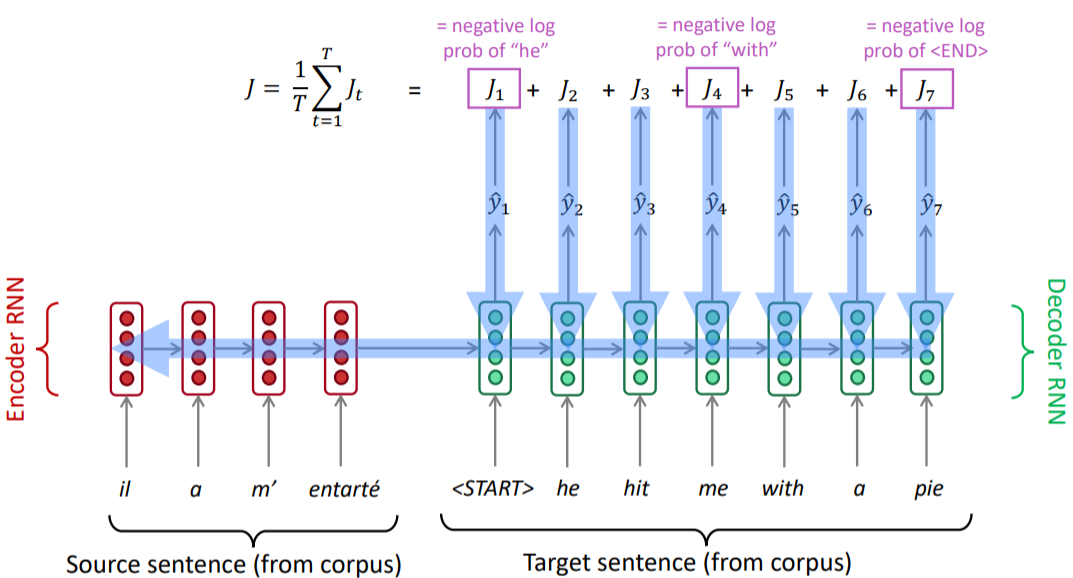
\includegraphics[width=8.0cm]{figs/NMT_training.png}}
	\caption{Training phase for NMT.}
	\label{fig:NMT_training}
\end{figure}

However, the aforementioned (greedy) decoding has no way to undo decisions. This is, if one of the output words are wrong, all the follow-up outputs are also wrong.
\concept{Beam search} decoding is utilized to fix this problem: on each step of decoder, keep track of the $k$ (in practice around $5$ to $10$) most probable partial translation (\emph{hypotheses}, path, or branch).
The target is the path with the largest cumulative log probabilities with shortest one (i.e. average).
Apart from all paths reach <END> as the stop sign, we can set some pre-defined cutoff for maximum number of timesteps or finished paths.

Although NMT is much simple and less human engineering effort while achieves better performance, NMT is diffcult to control (i.e. specify rules or guidelines) and less interpretable which leads to hard to debug.

The popular evaluation metric for MT is \concept{BLEU} (Bilingual Evaluation Understudy).
Its calculation is based on n-gram precision plus a penality for too-short translations.
Note that BLEU is useful but imperfect because there are many valid translations which has low $n$-gram overlap with the ground truth translation.
NMT outperforms SMT quickly, but there are still many difficulties remain:
\begin{itemize}
	\item Out-of-vocabulary words.
	\item Domain mismatch between train and test data.
	\item Maintaining context over longer text (long-term dependencies).
	\item Low-resource language pairs (few-shot learning).
	\item Using common sense is still hard.
\end{itemize}

\begin{figure}[!thp]
	\centerline{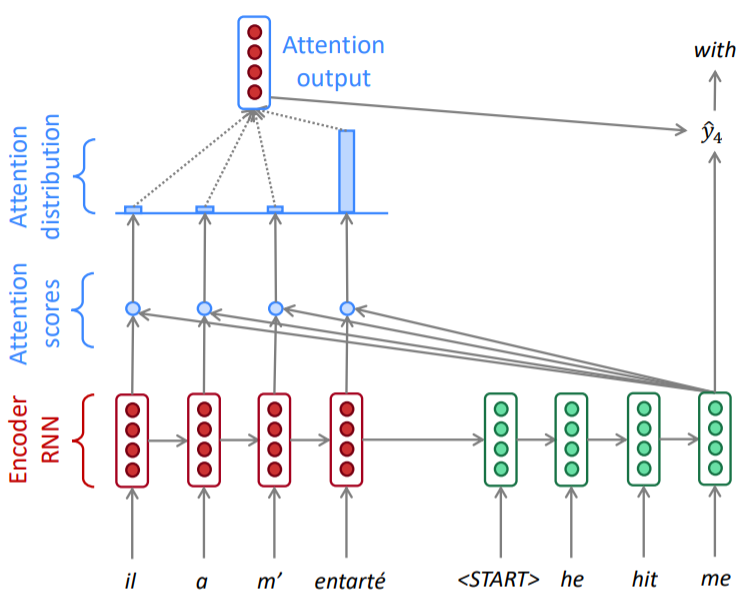
\includegraphics[width=8.0cm]{figs/Seq2Seq_attention.png}}
	\caption{Seq2Seq with attention.}
	\label{fig:Seq2Seq_Attention}
\end{figure}

We notice that only the last hidden state from encoder RNN to represent the whole source sentence may be the information bottleneck.
Thus we introduce Seq2Seq with \concept{attention}: on each step of the decoder, we use the attention distribution (like soft version of alignment) for each hidden states of encoder RNN to take a weighted sum of the encoder hidden states as the current decoder hidden state.
Note that sometimes the input of decoder RNN will concatenate the previous translated word vector and the previous attention output.
The diagram can be seen in Fig.\ref{fig:Seq2Seq_Attention}.
In addition, attention in here helps with vanishing gradient problem by providing shortcut to faraway states, and also provides some interpretability.
More formally, the attention for Seq2Seq is:
\begin{align}
&\bm{e}^{(t)} = [\bm{s}_t^\top \bm{h}_1, \cdots, \bm{s}_t^\top \bm{h}_n] \in \mathbb{R}^n \nonumber \\
&\text{Attention distribution: } \bm{\alpha}^{(t)} = \texttt{softmax}(\bm{e}^{(t)}) \nonumber \\
&\text{Attention output: } \bm{a}^{(t)} = \sum_{i=1}^n \alpha_i^{(t)} \bm{h}_i \in \mathbb{R}^h \nonumber \\
&\text{Attention decoder hidden state: } [\bm{a}^{(t)}; \bm{s}_t] \in \mathbb{R}^{2h}
\end{align}
where encoder hidden states $\bm{h}_1, \cdots, \bm{h}_n \in \mathbb{R}^h$, and decoder hidden state at timestep $t$ is $\bm{s}_t \in \mathbb{R}^h$.

More general definition of attention: given a set of vector \emph{values}, and a vector \emph{query}, attention is to compute a weighted sum of the values, dependent on the query.
We can found that attention is a way to obtain a \emph{fixed-size} representation of an arbitrary set of representations (e.g. sequential features).
There are many ways to obtain query vector: dot product $e_i = \bm{s}^\top \bm{h}_i$, multiplicative $e_i = \bm{s}^\top \bm{W} \bm{h}_i$, additive $e_i = \bm{v}^\top \tanh (\bm{W}_1 \bm{h}_i + \bm{W}_2 \bm{s})$, where $\bm{v}, \bm{W}, \bm{W}_1, \bm{W}_2$ are trainable parameters.

As for \emph{out-of-vocabulary} (OOV) problem in NMT, we can increase the size of vocabulary.
However, large vocabulary leads to huge computations in the softmax layer.
To solve it, we can use \emph{hierarchical softmax} (tree-structured vocabulary).
We can also use character-based model instead of word-based to handle OOV problem.

\subsection{HW4}
\textbf{1. Neural Machine Translation with RNNs}

Refer to the source codes for detail.
Note that \href{https://stackoverflow.com/questions/51030782/why-do-we-pack-the-sequences-in-pytorch}{pack\_padded\_sequence} is often used to reduce unnecessary computations of paded elements for variable length sequence.
In implementation, I found that for reshaping the last\_hidden with shape (2, b, h) to shape (b, 2h), I had to use \texttt{torch.cat((last\_hidden[0, :], last\_hidden[1, :]), axis=1)} instead of \texttt{.permute(1, 0, 2).view(b, -1)}.
Common used torch function include: \texttt{torch.squeeze}, \texttt{torch.unsqueeze}, \texttt{torch.split}, \texttt{torch.cat}, \texttt{torch.stack}, \texttt{torch.Tensor.view}, \texttt{torch.Tensor.permute}, \texttt{torch.Tensor.size}.

(i) Corpus BLEU score when testing: $22.68$.

(j) Dot product attention is simple but requires $\bm{s}_t, \bm{h}_i$ have the same shape. Additive attention could learn more complicated features but need more computations. 

\textbf{2. Analyzing NMT Systems}

(a)
\begin{enumerate}[label=(\roman*)]
	\item Error: duplication of translations ("favorite"), Reason: model limitations in preventing duplications, Solution: add penalty on duplicated translations.
	\item Error: the superlative comparison is mistranslated (most instead of more), Reason: could be because specific linguistic construct of comparison in Spanish, Solution: train with more comparision examples or add penalty for comparision examples.
	\item Reason: out-of-vocabulary words of names, Reason: the model do not consider out-of-vocabulary words, Solution: keep the out-of-vocabulary the same according to named entity regconization or attention output, or just increase the size of vocabulary.
	\item Error: "go around" is mistranslated to "go back," "block" is mistranslated to "apple", Reason: "apple" and "block" are same in Spanish "manzana", "go around" and "go back" are also similar in Spanish, Solution: train with more examples about such polysemic words.
	\item Error: "teacher" is mistranslated to "women" for Spanish "profesores", Reason: training dataset may contain the above mistakes, Solution: correct the dataset and add rules to correct this error.
	\item Error: "hectareas" (1/4 acres) is mistranslated to "acres", Reason: there is no such measure unit in English, Solution: identify measure unit in the source sentence and perform some rules.
\end{enumerate}

(b)

\sidenotedcmmc{Note that despite the HW taking sentence-level BLEU, BLEU is used as a \concept{corpus-level measure}.}

(c) BLEU
\begin{enumerate}[label=(\roman*)]
	\item $p_1 = 0.5477, p_2 = 0.6325$, $c_2$, agree.
	\item $p_1 = 0.4484, p_2 = 0.2589$, $c_1$, disagree.
	\item There are often many valiad translations for one sentence.
	\item Pros and cons of BELU:
	\begin{itemize}
		\item Pros: 1. BLEU has frequently been reported as correlating well with human judgement. 2. few human effort with inexpensive computations.
		\item Cons: 1. A good translation can get a poor BLEU score because it has low n-gram overlap with the human (reference) translation. 2. It does not consider meaning and sentence structure, etc.
	\end{itemize}
\end{enumerate}

\subsection{Tips for Research}
Two basic start points:
\begin{itemize}
	\item Start with a (domain) problem of interest and try to find good/better ways to address it than currently known/used.
	\item Start with a technical approach of interest, and work out good ways to extend or improve it or new ways to apply it.
	\item Experimental strategy: start from simple model and work incrementally on models, initially run on a tiny dataset (e.g. $8$ exmaples), make sure get $100\%$ accuracy on testing, then run your model on a large dataset that still get score to $100\%$ on training (it's okay to overfitting), and try to regularize the model.
\end{itemize}

Recommendation sources: ACL, NeurIPS, ICML, ICLR, arXiv (\href{http://www.arxiv-sanity.com/}{arXiv-sanity}), \href{https://paperswithcode.com/}{PapersWithCode} (leaderboards for various tasks).

\section{Contextual Word Representations and Pretraining} \label{contextual_word_rep}

\section{Attention Model and Question Answering}

Compared with previous versions, Stanford Question Answering Dataset (SQuAD) 2.0 has many unanswerable questions.
Each question has 3 gold answers, and there are two evaluation metrics:
\begin{itemize}
	\item Exact match (EM): 1/0 accuracy on whether match one of 3 answers.
	\item F1: take system (predict) and gold answers as bag of words to calculate F1 scores.
\end{itemize}
where both metrics ignore punctuation and articles.
Disadvantages:  the answer is only sub-span of the paragraph (the answers are directly appeared in the question), without indirect answers, e.g., yes/no, counting, and implicit why.

A simple and successful aechitecture is the Stanford Attentive Reader \mycite{SAR} which likes the attentive Seq2Seq model.
For paragraph $[\bm{p}_1, \cdots, \bm{p}_m]$ and question $[\bm{q}_1, \cdots, \bm{q}_n]$ with GloVe embedding, the index of start token and end token for the sub-span answer is:
\begin{align}
&\bm{q} = [\overrightarrow{\text{LSTM}}(\overrightarrow{\bm{h}}^{(m-1)}, \bm{q}_{m-1}); \overleftarrow{\text{LSTM}}(\overleftarrow{\bm{h}}^{(2)}, \bm{q}_{2})] \nonumber \\
&\tilde{\bm{p}}_i = \text{Bi-LSTM}(\bm{p}_i) \nonumber \\
&\text{Start token: } \text{softmax}_i (\bm{q}^\top \bm{W}_s \tilde{\bm{p}}_i) \nonumber \\
&\text{End token: } \text{softmax}_i (\bm{q}^\top \bm{W}_e \tilde{\bm{p}}_i) \nonumber
\end{align}

Compared with SAR, Stanford Attentive Reader++ \mycite{DrQA} mainly leverages these updates: (1) use weighted sum (attention) of all hidden states in the encoder of question, (2) multi-layers Bi-LSTM (3) add more features in the encoder of the paragraph, including linguistic features such as POS\&NER tags\&term frequency, exact match (wether the word appears in the question), aligned question embedding ($\sum_j \texttt{softmax}_{j^\prime}(\alpha(p_i) \cdot \alpha(q_{j^\prime})) \times q_j$ where $\alpha$ is dense layer with ReLU activation and $p_i, q_j$ are embedding of the paragraph and the question word.

Bi-Directional Attention Flow (DiDAF) \mycite{BiDAF} is a state-of-the-art (SoTA) method in 2018 and 2017.
It comes up with word and char embedding, and the main innovation is attention flow layer which consists of Query2Context (i.e. Question2Paragraph) and Context2Query.
C2Q attention is defined as:
\begin{align}
&\text{Similarity matrix: } s_{ij} = w_s^\top [p_i; q_j; p_i \circ q_j] \in \mathbb{R} \\
&\alpha_i = \text{softmax}(s_{i,:}) \\
&a_i = \sum_j \alpha_{ij} q_j \in \mathbb{R}^{2h} 
\end{align}

\begin{figure}[!thp]
	\centerline{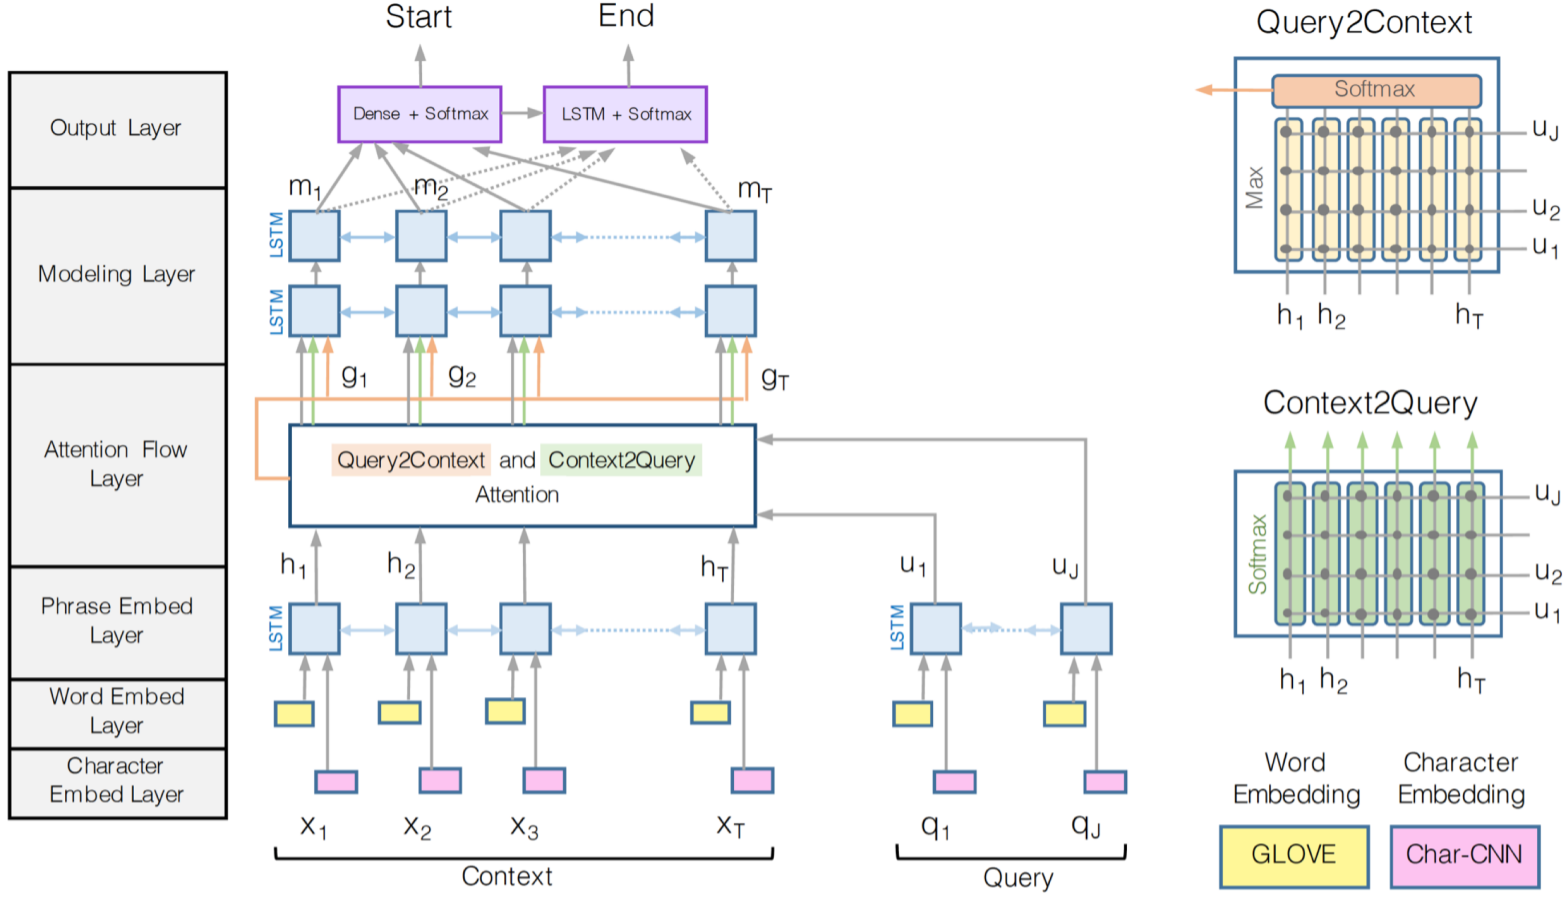
\includegraphics[width=8.0cm]{figs/BiDAF.png}}
	\caption{Architecture of BiDAF}
	\label{fig:bidaf}
\end{figure}

Q2C attention (the weighted sum of the most important words in the context w.r.t the query) is given by:
\begin{align}
&m_i = \max_j s_{ij} \\
&\beta = \text{softmax}(m) \\
&p^\prime = \sum_i \beta_i p_i
\end{align}
The BiDAF layer output of each paragraph position is: $b_i = [p_i; a_i; p_i \circ a_i; p_i \circ p^\prime] \in \mathbb{R}^{8h}$.
The overall architecture is presented in Fig.\ref{fig:bidaf}.
The start token comes from the output of dense layer with softmax built upon the concatenation of the BiDAF output and the output $M_1$ of modelling layer (2-layer Bi-LSTM) whose input is BiDAF output.
And the end token is the dense layer with softmax upon the concatenation of the BiDAF output and the output $M_2$ of another modelling layer whose input is $M_1$.

\section{ConvNets for NLP}

Convolutions are classically used to extract (position-invariant) features from images by leveraging fixed-size \emph{filter} (\emph{kernel}) weights which are used to perform element-wise product with certain window (patch) of the whole image.
\emph{Zero padding} ("same" padding) is often used to keep the length.
The kernel window slides with a stride (e.g. 1) over the whole sentence.
One more variant about convolutions is \emph{dilation convolution} (skip conv) which can access more wide \emph{receptive field} with smaller filter.
Same as the \emph{channels} (aka. feature maps) in CNNs, we can also define the dimensions of word embedding as channels like 3 channels (RBG) of images.
Each channel may indicates one feature (e.g. words about food or sport).
\emph{Pooling} (e.g. max, average) over time (aka. global pooling) is utilized to aggregate the information of the whole sentence.
$k$-max (global) pooling is also a common technique used in ConvNet for NLP.
Besides, local pooling is more common used in CNN circumstances.
1x1 convolution (aka. Network-in-Network connection) is a famous technique that can be seen as a fully connection linear layer across chennels.
It can be also (often) used to map from many channels to fewer channels to reduce computation while keeping performance.

\begin{figure}[!thp]
	\centerline{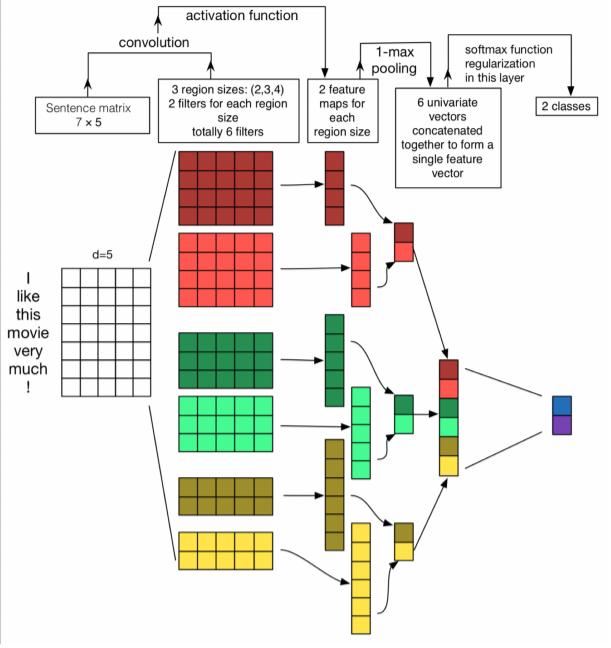
\includegraphics[width=10.0cm]{figs/ConvNet_NLP.png}}
	\caption{Simple ConvNet for NLP classification.}
	\label{fig:ConvNetNLP}
\end{figure}

Above is an example \mycite{kim-2014-convolutional} of single layer CNN for sentence classification.
Fig.\ref{fig:ConvNetNLP} illustrates the architecture.
Multiple single convolution layer with different kernel size and global max pooling are used.
Specifically, there are 100 feature maps for each of kernel size 3, 4, and 5. 
The input is two copies of pre-trained word vector (word2vec-300).
Keep one as 'static' (no gradient), and the other 'dynamic' will be updated during training.
The 'static' word vector gives unseen words appeared in the test set a better chance of being interreted correctly.
There are several ways of handling these two channels, most common is to simply average them before using in a CNN.
The other method is to double the length of the CNN filters.
The output of max poolings are concatenated into a vector, which is then fed into a dense layer with softmax to perform classification.
Dropout and L2 regularization are used.

VD-CNN \mycite{VDCNN} for text classification is to build a ResNet like very deep CNN which has 29 depth and many shortcut (residual) connections.
Note that 29 depth is not as deep as ResNet whose depths are typically 34, 50, and 101.
The researchers found that, for more deep one like 47 layers, the results are fraction worse than the one with 29 layers.
The input text sequence will pad into fixed length (1024).

Quasi-recurrent neural network takes the best and parallelizable parts of RNNs and CNNs.
It achives $3\sim16$ times faster than LSTM.
One Quasi-RNN layer consists of a normal convolution layer with left same padding to learn new hidden content $z$, forget gate $f$, optional output gate $i$, and optional input gate $i$, and three dynamic average pooling (non-parametric) variants to perform RNN-like unfolding.
\begin{align}
&\text{New hidden contents: } \bm{Z} = \tanh(\bm{W}_z * \bm{X}) \nonumber \\
&\text{Forget gates: } \bm{F} = \sigma(\bm{W}_f * \bm{X}) \nonumber \\
&\text{Optional output gates: } \bm{O} = \sigma(\bm{W}_o * \bm{X}) \nonumber \\
&\text{Optional input gates: } \bm{I} = \sigma(\bm{W}_i * \bm{X}) \nonumber \\
&\textit{f}\text{-pooling: } \bm{h}_t = \bm{f}_t \odot \bm{h_{t-1}} + (1 - \bm{f}_t) \odot \bm{z}_t \nonumber \\
&\textit{fo}\text{-pooling: } \nonumber \\
\begin{split}
&\bm{c}_t = \bm{f}_t \odot \bm{c}_{t-1} + (1-\bm{f}_t) \odot \bm{z}_t) \nonumber \\
&\bm{h}_t = \bm{o}_t \odot \bm{c}_t \nonumber
\end{split} \nonumber \\
&\textit{ifo}\text{-pooling: } \nonumber \\
\begin{split}
&\bm{c}_t = \bm{f}_t \odot \bm{c}_{t-1} + \bm{i}_t \odot \bm{z}_t) \nonumber \\
&\bm{h}_t = \bm{o}_t \odot \bm{c}_t \nonumber
\end{split} \nonumber
\end{align}
where the hidden state $\bm{h}$ and the cell state $\bm{c}$ are initialized to zeros, $*$ indicates convolution operator, and $\odot$ denotes element-wise product.
A variant dropout called zoneout is adopt in the forget gate channels of stacked QRNN.
Dense connection layers from DenseNet are also extended in stacked QRNN.
Note that QRNN often need deeper network to get as good performance as LSTM.

\section{Subword models}

Although what our mouths produce is continuous space, phonology posits phonetics the sound stream that consists of smaller distinctive categorical units: phonemes.
In linguistics, morphemes (subwords) is the smallest semantic unit that has meanings, e.g. unfortunately can be divided into tree structure of morephemes using \emph{recursive neural networks} \mycite{morphology}:

\begin{equation}
[[\text{un }[[\text{fortun(e)}]_{\text{ROOT}} \text{ ate}]_{\text{STEM}}]_{\text{STEM}}\text{ ly}]_{\text{WORD}} \nonumber
\end{equation}

There are many languages that do not segment words or has many separated and joined words, e.g. Chinese, French.
Moreover, subword models solve the OOV problem.
